\begin{figure}[htb]
\begin{center}
\def\svgwidth{10cm}
% GNUPLOT: LaTeX picture with Postscript
\begingroup
  \makeatletter
  \providecommand\color[2][]{%
    \GenericError{(gnuplot) \space\space\space\@spaces}{%
      Package color not loaded in conjunction with
      terminal option `colourtext'%
    }{See the gnuplot documentation for explanation.%
    }{Either use 'blacktext' in gnuplot or load the package
      color.sty in LaTeX.}%
    \renewcommand\color[2][]{}%
  }%
  \providecommand\includegraphics[2][]{%
    \GenericError{(gnuplot) \space\space\space\@spaces}{%
      Package graphicx or graphics not loaded%
    }{See the gnuplot documentation for explanation.%
    }{The gnuplot epslatex terminal needs graphicx.sty or graphics.sty.}%
    \renewcommand\includegraphics[2][]{}%
  }%
  \providecommand\rotatebox[2]{#2}%
  \@ifundefined{ifGPcolor}{%
    \newif\ifGPcolor
    \GPcolortrue
  }{}%
  \@ifundefined{ifGPblacktext}{%
    \newif\ifGPblacktext
    \GPblacktextfalse
  }{}%
  % define a \g@addto@macro without @ in the name:
  \let\gplgaddtomacro\g@addto@macro
  % define empty templates for all commands taking text:
  \gdef\gplbacktext{}%
  \gdef\gplfronttext{}%
  \makeatother
  \ifGPblacktext
    % no textcolor at all
    \def\colorrgb#1{}%
    \def\colorgray#1{}%
  \else
    % gray or color?
    \ifGPcolor
      \def\colorrgb#1{\color[rgb]{#1}}%
      \def\colorgray#1{\color[gray]{#1}}%
      \expandafter\def\csname LTw\endcsname{\color{white}}%
      \expandafter\def\csname LTb\endcsname{\color{black}}%
      \expandafter\def\csname LTa\endcsname{\color{black}}%
      \expandafter\def\csname LT0\endcsname{\color[rgb]{1,0,0}}%
      \expandafter\def\csname LT1\endcsname{\color[rgb]{0,1,0}}%
      \expandafter\def\csname LT2\endcsname{\color[rgb]{0,0,1}}%
      \expandafter\def\csname LT3\endcsname{\color[rgb]{1,0,1}}%
      \expandafter\def\csname LT4\endcsname{\color[rgb]{0,1,1}}%
      \expandafter\def\csname LT5\endcsname{\color[rgb]{1,1,0}}%
      \expandafter\def\csname LT6\endcsname{\color[rgb]{0,0,0}}%
      \expandafter\def\csname LT7\endcsname{\color[rgb]{1,0.3,0}}%
      \expandafter\def\csname LT8\endcsname{\color[rgb]{0.5,0.5,0.5}}%
    \else
      % gray
      \def\colorrgb#1{\color{black}}%
      \def\colorgray#1{\color[gray]{#1}}%
      \expandafter\def\csname LTw\endcsname{\color{white}}%
      \expandafter\def\csname LTb\endcsname{\color{black}}%
      \expandafter\def\csname LTa\endcsname{\color{black}}%
      \expandafter\def\csname LT0\endcsname{\color{black}}%
      \expandafter\def\csname LT1\endcsname{\color{black}}%
      \expandafter\def\csname LT2\endcsname{\color{black}}%
      \expandafter\def\csname LT3\endcsname{\color{black}}%
      \expandafter\def\csname LT4\endcsname{\color{black}}%
      \expandafter\def\csname LT5\endcsname{\color{black}}%
      \expandafter\def\csname LT6\endcsname{\color{black}}%
      \expandafter\def\csname LT7\endcsname{\color{black}}%
      \expandafter\def\csname LT8\endcsname{\color{black}}%
    \fi
  \fi
  \setlength{\unitlength}{0.0500bp}%
  \begin{picture}(7200.00,5040.00)%
    \gplgaddtomacro\gplbacktext{%
      \csname LTb\endcsname%
      \put(1474,704){\makebox(0,0)[r]{\strut{} 1.2e+11}}%
      \put(1474,1286){\makebox(0,0)[r]{\strut{} 1.3e+11}}%
      \put(1474,1867){\makebox(0,0)[r]{\strut{} 1.4e+11}}%
      \put(1474,2449){\makebox(0,0)[r]{\strut{} 1.5e+11}}%
      \put(1474,3030){\makebox(0,0)[r]{\strut{} 1.6e+11}}%
      \put(1474,3612){\makebox(0,0)[r]{\strut{} 1.7e+11}}%
      \put(1474,4193){\makebox(0,0)[r]{\strut{} 1.8e+11}}%
      \put(1474,4775){\makebox(0,0)[r]{\strut{} 1.9e+11}}%
      \put(1606,484){\makebox(0,0){\strut{} 5}}%
      \put(2256,484){\makebox(0,0){\strut{} 6}}%
      \put(2905,484){\makebox(0,0){\strut{} 7}}%
      \put(3555,484){\makebox(0,0){\strut{} 8}}%
      \put(4205,484){\makebox(0,0){\strut{} 9}}%
      \put(4854,484){\makebox(0,0){\strut{} 10}}%
      \put(5504,484){\makebox(0,0){\strut{} 11}}%
      \put(6153,484){\makebox(0,0){\strut{} 12}}%
      \put(6803,484){\makebox(0,0){\strut{} 13}}%
      \put(176,2739){\rotatebox{-270}{\makebox(0,0){\strut{}Spezifische Elektronenladung $\nicefrac{e}{m_e}\,[\unitfrac{C}{kg}]$}}}%
      \put(4204,154){\makebox(0,0){\strut{}Durchmesser der Elektronenkreisbahn $d\,[\unit{cm}]$}}%
    }%
    \gplgaddtomacro\gplfronttext{%
      \csname LTb\endcsname%
      \put(5816,1317){\makebox(0,0)[r]{\strut{}Konst. Magnetfeld}}%
      \csname LTb\endcsname%
      \put(5816,1097){\makebox(0,0)[r]{\strut{}Elliptische Integrale}}%
      \csname LTb\endcsname%
      \put(5816,877){\makebox(0,0)[r]{\strut{}Literaturwert}}%
    }%
    \gplbacktext
    \put(0,0){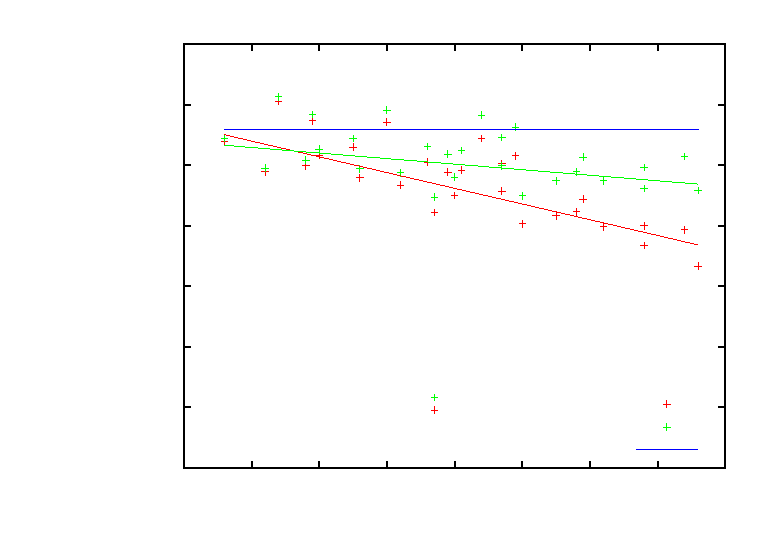
\includegraphics{ergebnisse}}%
    \gplfronttext
  \end{picture}%
\endgroup

\end{center}
\caption{Ergebnisse der Bestimmung der spezifischen Elektronenladung}
\label{fig:ergebnisse}
\end{figure}
Da die Abweichung des ermittelten Wertes mit $7.3\,\%$ außerhalb des ermittelten Fehlerbereichs liegt, scheinen die verwendeten Abschätzungen unzureichend zu sein.

Eine noch nicht betrachtete Fehlerquelle ist die Annahme des homogenen Magnetfeldes im Bereich des Glaskolbens.
Diese Näherung führt zu einer recht großen Abweichung, wie die Berechnung des Wertes mit elliptischen Integralen\footnote{per Wolfram Mathematica$^\text{\textregistered}$} zeigt. Die dafür benötigten Formeln wurden der Praktikumsanleitung \citep[S.~108]{Anleitung} entnommen.
Die relative Abweichung vom Literaturwert beträgt dann nur noch etwa $3.3\,\%$. Ein Vergleich der Ergebnisse ist in Abbildung~\ref{fig:ergebnisse} zu sehen. Auch gut zu erkennen ist die steigende Abweichung mit größerem Radius der Elektronenkreisbahn.
%Eine Berechnung des Fehlers per Gaußscher Fehlerfortpflanzung\footnote{mit Hilfe von Wolfram Mathematica$^\text{\textregistered}$} ergibt einen maximalen Messfehler von $\unit[?]{A}$.
Leider gestaltet sich die Berechnung der Gaußschen Fehlerfortpflanzung bei elliptischen Integralen äußerst schwierig, sodass darauf verzichtet werden musste.

Eine weitere Möglichkeit, die spezifische Elektronenladung aus den Messwerten zu bestimmen, ist das graphische Auftragen der Messwerte (siehe Abb.~\ref{fig:dUI-Kackplot}) mit anschließendem Ablesen der Steigung.
\begin{figure}[htb]
\begin{center}
\def\svgwidth{8cm}
% GNUPLOT: LaTeX picture with Postscript
\begingroup
  \makeatletter
  \providecommand\color[2][]{%
    \GenericError{(gnuplot) \space\space\space\@spaces}{%
      Package color not loaded in conjunction with
      terminal option `colourtext'%
    }{See the gnuplot documentation for explanation.%
    }{Either use 'blacktext' in gnuplot or load the package
      color.sty in LaTeX.}%
    \renewcommand\color[2][]{}%
  }%
  \providecommand\includegraphics[2][]{%
    \GenericError{(gnuplot) \space\space\space\@spaces}{%
      Package graphicx or graphics not loaded%
    }{See the gnuplot documentation for explanation.%
    }{The gnuplot epslatex terminal needs graphicx.sty or graphics.sty.}%
    \renewcommand\includegraphics[2][]{}%
  }%
  \providecommand\rotatebox[2]{#2}%
  \@ifundefined{ifGPcolor}{%
    \newif\ifGPcolor
    \GPcolortrue
  }{}%
  \@ifundefined{ifGPblacktext}{%
    \newif\ifGPblacktext
    \GPblacktextfalse
  }{}%
  % define a \g@addto@macro without @ in the name:
  \let\gplgaddtomacro\g@addto@macro
  % define empty templates for all commands taking text:
  \gdef\gplbacktext{}%
  \gdef\gplfronttext{}%
  \makeatother
  \ifGPblacktext
    % no textcolor at all
    \def\colorrgb#1{}%
    \def\colorgray#1{}%
  \else
    % gray or color?
    \ifGPcolor
      \def\colorrgb#1{\color[rgb]{#1}}%
      \def\colorgray#1{\color[gray]{#1}}%
      \expandafter\def\csname LTw\endcsname{\color{white}}%
      \expandafter\def\csname LTb\endcsname{\color{black}}%
      \expandafter\def\csname LTa\endcsname{\color{black}}%
      \expandafter\def\csname LT0\endcsname{\color[rgb]{1,0,0}}%
      \expandafter\def\csname LT1\endcsname{\color[rgb]{0,1,0}}%
      \expandafter\def\csname LT2\endcsname{\color[rgb]{0,0,1}}%
      \expandafter\def\csname LT3\endcsname{\color[rgb]{1,0,1}}%
      \expandafter\def\csname LT4\endcsname{\color[rgb]{0,1,1}}%
      \expandafter\def\csname LT5\endcsname{\color[rgb]{1,1,0}}%
      \expandafter\def\csname LT6\endcsname{\color[rgb]{0,0,0}}%
      \expandafter\def\csname LT7\endcsname{\color[rgb]{1,0.3,0}}%
      \expandafter\def\csname LT8\endcsname{\color[rgb]{0.5,0.5,0.5}}%
    \else
      % gray
      \def\colorrgb#1{\color{black}}%
      \def\colorgray#1{\color[gray]{#1}}%
      \expandafter\def\csname LTw\endcsname{\color{white}}%
      \expandafter\def\csname LTb\endcsname{\color{black}}%
      \expandafter\def\csname LTa\endcsname{\color{black}}%
      \expandafter\def\csname LT0\endcsname{\color{black}}%
      \expandafter\def\csname LT1\endcsname{\color{black}}%
      \expandafter\def\csname LT2\endcsname{\color{black}}%
      \expandafter\def\csname LT3\endcsname{\color{black}}%
      \expandafter\def\csname LT4\endcsname{\color{black}}%
      \expandafter\def\csname LT5\endcsname{\color{black}}%
      \expandafter\def\csname LT6\endcsname{\color{black}}%
      \expandafter\def\csname LT7\endcsname{\color{black}}%
      \expandafter\def\csname LT8\endcsname{\color{black}}%
    \fi
  \fi
  \setlength{\unitlength}{0.0500bp}%
  \begin{picture}(7200.00,5040.00)%
    \gplgaddtomacro\gplbacktext{%
      \csname LTb\endcsname%
      \put(1078,704){\makebox(0,0)[r]{\strut{} 0.05}}%
      \put(1078,1213){\makebox(0,0)[r]{\strut{} 0.06}}%
      \put(1078,1722){\makebox(0,0)[r]{\strut{} 0.07}}%
      \put(1078,2231){\makebox(0,0)[r]{\strut{} 0.08}}%
      \put(1078,2740){\makebox(0,0)[r]{\strut{} 0.09}}%
      \put(1078,3248){\makebox(0,0)[r]{\strut{} 0.1}}%
      \put(1078,3757){\makebox(0,0)[r]{\strut{} 0.11}}%
      \put(1078,4266){\makebox(0,0)[r]{\strut{} 0.12}}%
      \put(1078,4775){\makebox(0,0)[r]{\strut{} 0.13}}%
      \put(1210,484){\makebox(0,0){\strut{} 12}}%
      \put(2009,484){\makebox(0,0){\strut{} 14}}%
      \put(2808,484){\makebox(0,0){\strut{} 16}}%
      \put(3607,484){\makebox(0,0){\strut{} 18}}%
      \put(4406,484){\makebox(0,0){\strut{} 20}}%
      \put(5205,484){\makebox(0,0){\strut{} 22}}%
      \put(6004,484){\makebox(0,0){\strut{} 24}}%
      \put(6803,484){\makebox(0,0){\strut{} 26}}%
      \put(176,2739){\rotatebox{-270}{\makebox(0,0){\strut{}$d\,[\unit{m}]$}}}%
      \put(4006,154){\makebox(0,0){\strut{}$\sqrt{\frac{U}{\unit{1}{V}}}/\frac{I}{\unit{1}{A}}\,[\sim]$}}%
    }%
    \gplgaddtomacro\gplfronttext{%
      \csname LTb\endcsname%
      \put(5816,4602){\makebox(0,0)[r]{\strut{}Messwerte}}%
      \csname LTb\endcsname%
      \put(5816,4382){\makebox(0,0)[r]{\strut{}Lineare Regression}}%
    }%
    \gplbacktext
    \put(0,0){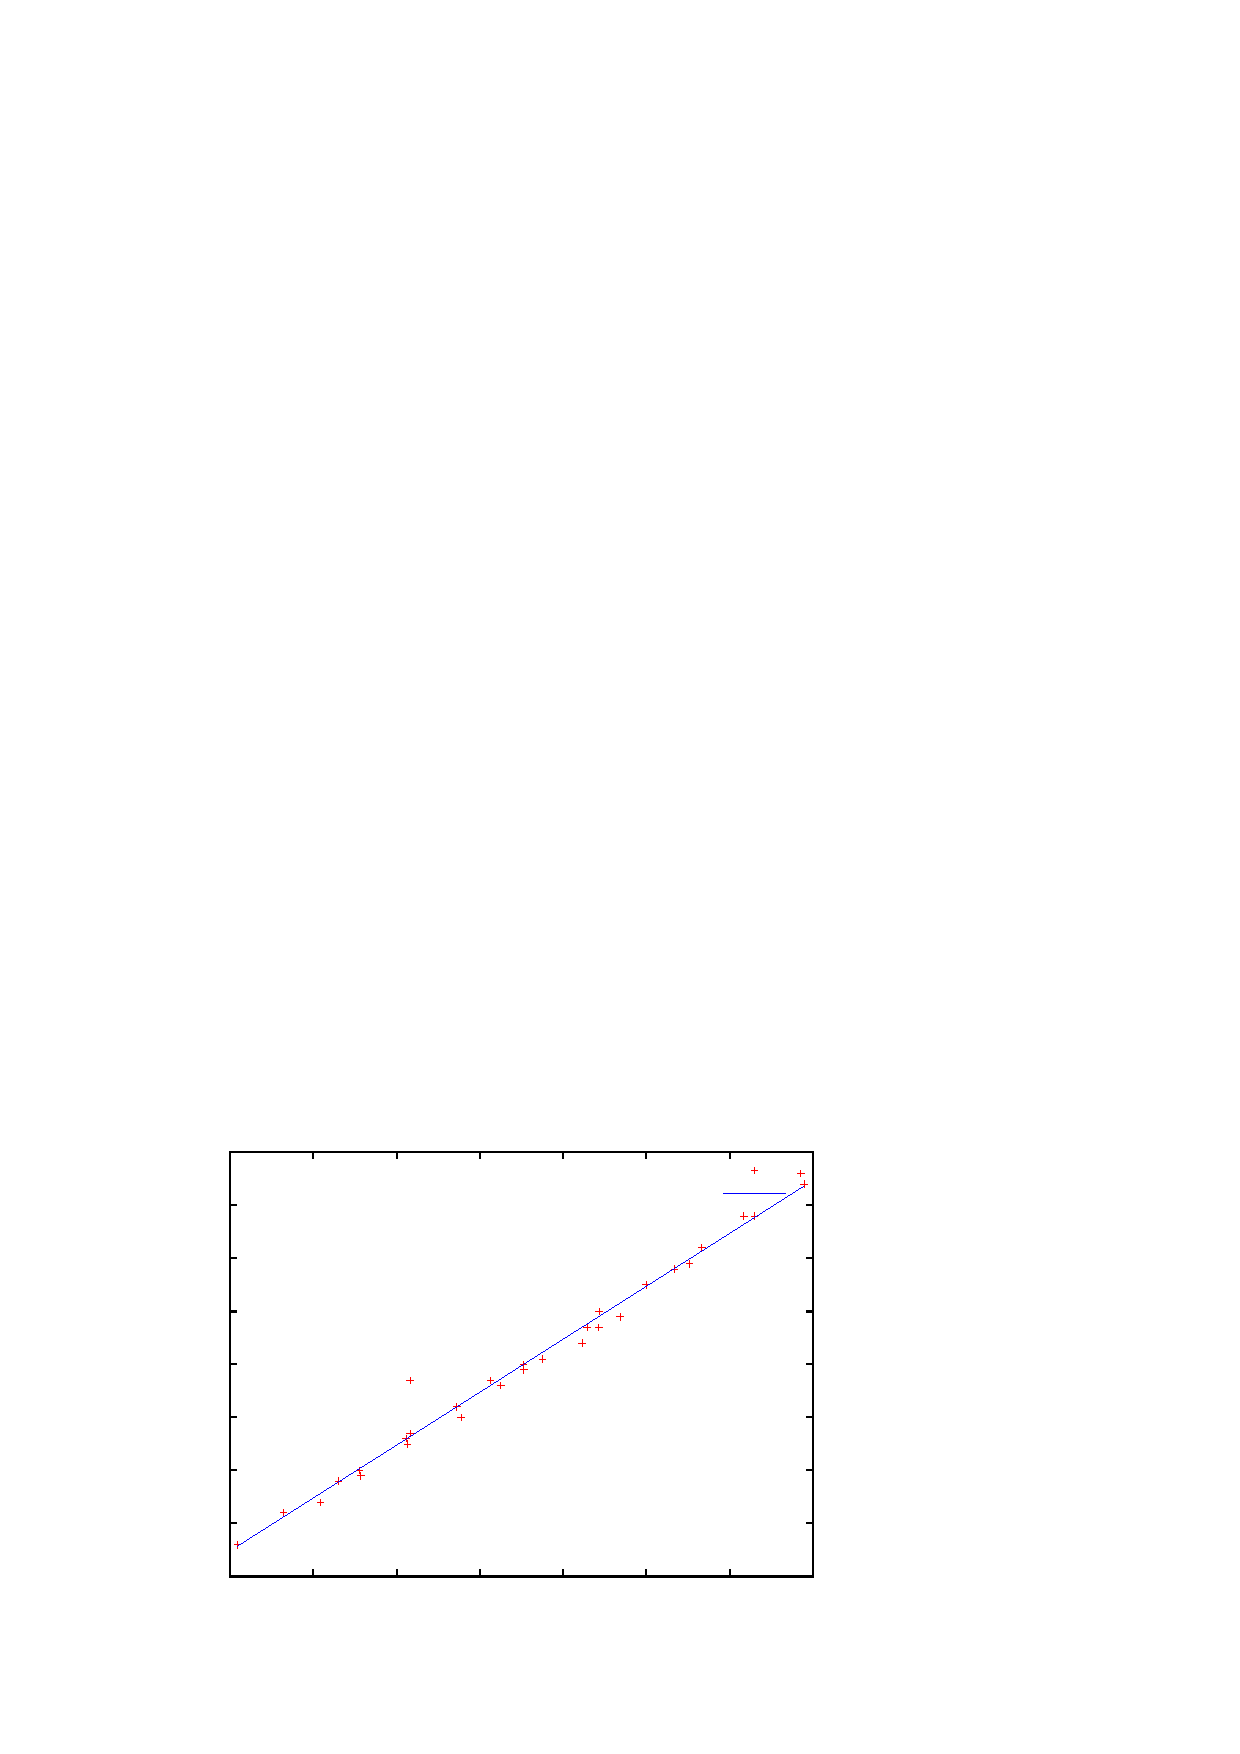
\includegraphics{edurchm}}%
    \gplfronttext
  \end{picture}%
\endgroup

\end{center}
\caption{Abhängigkeit des Elektronenstrahldurchmessers $d$ von dem Quotienten aus der Quadratwurzel der Spannung und der Stromstärke $\sqrt{U}/I$.}
\label{fig:dUI-Kackplot}
\end{figure}
Aus den Formeln~\ref{eq:B-Feld} und~\ref{eq:SpezLad} kann dann durch einfaches Umstellen und Einsetzen der Steigung ein Wert für die spezifische Ladung bestimmt werden.
Die relative Abweichung vom Literaturwert beträgt jedoch etwa $\unit[15.9]{\%}$.
Diese Berechnungsmethode führt also vermutlich zu sehr viel schlechteren Werten als die Berechnung mit Hilfe der einzelnen Wertepaare und anschließender gewichteter Mittelung.

Dies ist sehr erfreulich, da sich offenbar der sehr viel höhere Aufwand der anderen Methoden gelohnt hat.
Zum Vergleich der drei verwendeten Verfahren untereinander und mit dem Literaturwert siehe auch Tabelle~\ref{tab:Vergleich}.

Es fällt auf, dass die berechneten Werte unabhängig von der Rechenmethode eine Abweichung nach unten aufweisen.

Es scheint also ein systematischer Fehler in der Messung vorzuliegen.
Dieser könnte zur Ursache haben, dass der Versatz der Längenskala zur Messung des Strahldurchmessers nur einmal gemessen wurde.
Hier würde eine Abweichung des Messwertes nach oben die beobachteten Konsequenzen nach sich ziehen.
In Frage käme außerdem noch ein schwächeres Magnetfeld als berechnet oder eine stärkere Spannung als gemessen.
Letzteres ist aufgrund der hohen Genauigkeit der Multimeter jedoch recht unwahrscheinlich.


Weiterhin könnte eine etwaige Brechung des Lichts durch den Glaskolben zu kleineren Ungenauigkeiten führen.
Auch eine mögliche bei Verschiebung des Okulars auftretende kleine Drehung desselben um die vertikale Achse würde eine zusätzliche Abweichung zur Folge haben.

Einer der Messwerte (für $U_\mathrm{B} = \unit[140]{V},\,I = \unit[725]{mA}$) fällt vollkommen aus der Reihe und ist in allen Diagrammen deutlich zu erkennen. Wenn man anstatt der notierten $\unit[11.4]{cm}$ jedoch $\unit[10.4]{cm}$ einsetzt, ergibt sich ein deutlich besserer Wert, der statt $\unit[25.2]{\%}$ nur um $\unit[4.4]{\%}$ abweicht. Hier ist den Experimentatoren also offenbar ein Fehler unterlaufen.
